\section{GPU based In-Situ Visualization Architecture}
Wong et al.~\cite{wong2012top} list top 10 challenges of extreme-scale visual analysis, and \emph{in-situ} analysis ranks the top one. Compared with traditional approaches, in situ VA tries to perform as much analysis as possible while the datasets are in memory for reducing I/O cost. In scientific visualization, in-situ processing and visualization are the general methods for handling big data \cite{ma2007situ},  when I/O becomes the performance bottleneck. 
%The idea is that simulation and visualization code run simultaneously which can reduce the data transfer and storage costs. 
In this paper, we adopt \emph{in-situ} concept, and propose that 
\textbf{data processing and visualization code  run together to reduce the number of visual primitives transferring between GPU memory and main memory}. Thus, all code can run on the GPU to fully utilize GPU parallel resources.

\begin{figure}[htb]
	\centering
	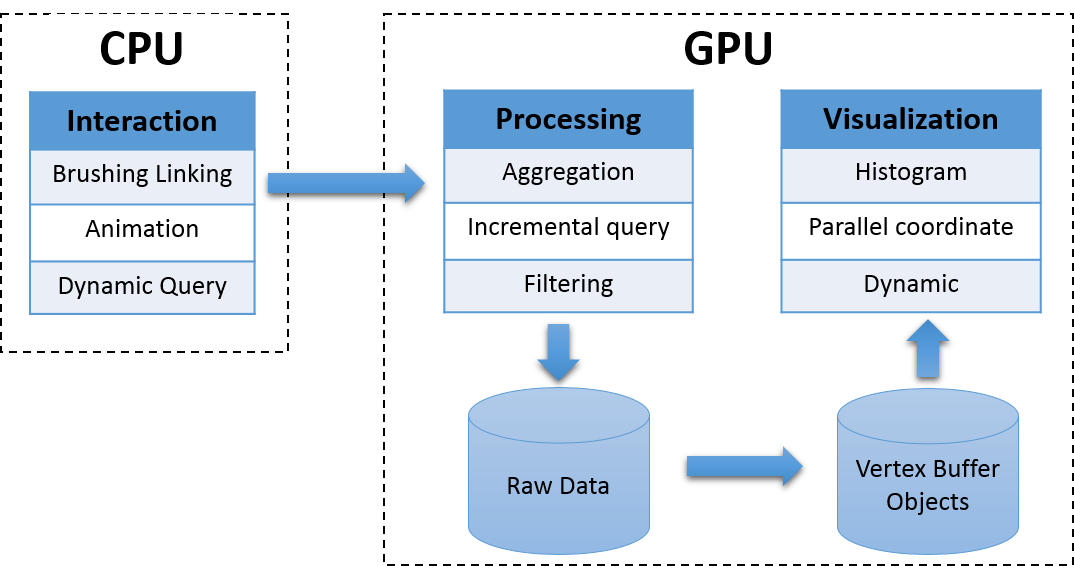
\includegraphics[width=1.0\linewidth]{pic/in-situ.png}
	\parbox[t]{1.0\columnwidth}{\relax
	}
	%
	\caption{\label{fig:architecture} The \emph{In-Situ} visualization architecture of the \emph{AVIST}.}
\end{figure}


Figure~\ref{fig:architecture} shows our GPU based in-situ visualization architecture, which incorporates previous mentioned visualization and interaction techniques. In the CPU sides, it only handles user interactions,  which trigger GPU parallel processing and rendering. The GPU controls all data transformation from  raw data into visualization results. It can process related queries and generate visual primitives simultaneous. All raw data is located in GPU memory to support users' drill-down query of each data record. All generated visual primitives are stored in GPU vertex buffer objects (VBO) to obtain substantial performance gains and avoid data transformation with main memory.
 


Our in-situ visualization architecture makes the best use of GPUs powerful computing and rendering performance. It supports filtering and visualizing items in parallel. More importantly, this kind of design avoids data transformation between main memory and GPU to reduce IO cost, which is potential bottleneck for big data VA systems. 


However, the major consideration of the in-situ visualization architecture is data scalability problem, which is limited by GPU memory capability. To feed more data into the GPU memory, we propose to preprocess datasets into compressed binary format.

%There are also two major considerations in our in-situ visualization architecture. The first one is that data size is limited by GPU memory size, the second is how to deploy incremental computing idea to gain better performance.

%\subsection{Data Preprocessing}
%In our architecture, the data size is limited by GPU memory capability. To feed more data into GPU memory, we preprocess the data into compressed binary format.

Considering general multi-dimensional datasets, we first identify each data type in datasets. For categorical and ordinal data, we count  all possible values and map each value into a unique ID. All values and their corresponding IDs are stored in main memory as meta-data. %While on the GPU memory, we just need to store each value's  corresponding ID. 
Then, we store datasets on GPU memory with their row-oriented format, which replaces the original values to  IDs  in binary format of one byte, two bytes or four bytes (e.g. if one dimension data only has less than 256 possible values, we can use one byte for representation.). For quantitative data, we simply store one \emph{Int} or \emph{Float} for representing each data value. We store  time data in \emph{$time\_t$} format, which occupies 8 bytes. Table \ref{preprocessing} summarizes our data preprocessing strategy. The row-oriented design targets temporal and spatial locality based analytical tasks for drilling-down query, which supports analysts to find  a ``needle in a haystack".  The preprocessing focuses on analyzing each column for compression and making sense of the whole datasets.


\begin{table}[h]
	\centering
	\caption{Data preprocessing methods}
	\label{preprocessing}
	\begin{tabular}{|c|c|c|}
		\hline
		\textbf{DataType}                                                     & \begin{tabular}[c]{@{}c@{}}\textbf{GPU memory}\\ \textbf{binary format}\end{tabular} & \begin{tabular}[c]{@{}c@{}} \textbf{Main memory} \\ \textbf{meta-data}\end{tabular}   \\ \hline
		Time                                                         & \begin{tabular}[c]{@{}c@{}}time\_t\\ 8 bytes\end{tabular}          & \begin{tabular}[c]{@{}c@{}}minimum\\  maximum\end{tabular}         \\ \hline
		Quantitative                                                 & \begin{tabular}[c]{@{}c@{}}Int or Float\\  4 bytes\end{tabular}    & \begin{tabular}[c]{@{}c@{}}minimum \\ maximum\end{tabular}         \\ \hline
		\begin{tabular}[c]{@{}c@{}}Categorial\\ Ordinal\end{tabular} & $1\sim4$ bytes                                                          & \begin{tabular}[c]{@{}c@{}}Dictionary\\ (IDs and data value)\end{tabular} \\ \hline
	\end{tabular}
\end{table}


A standard commercial graphics card has its memory from 4GB to 8GB. Considering a  dataset with most of its data attributes occupy 4 bytes, then the total data items we can handle is about 10 millions. So our VA system can handle million records in one GPU.